\documentclass[9pt,twocolumn,twoside]{osajnl}
%% Please use 11pt if submitting to AOP
% \documentclass[11pt,twocolumn,twoside]{osajnl}

\journal{josab} % Choose journal (ao, aop, josaa, josab, ol, optica, pr)

% See template introduction for guidance on setting shortarticle option
\setboolean{shortarticle}{false}
% true = letter / tutorial
% false = research / review article
% (depending on journal).

\usepackage{subcaption}
\usepackage{tikz}
\usepackage{mathtools}

\usetikzlibrary{patterns,decorations.pathreplacing}
\usetikzlibrary{arrows.meta}
\usetikzlibrary{shapes.arrows, fadings}

% Fixes bracket spacing
\let\originalleft\left
\let\originalright\right
\renewcommand{\left}{\mathopen{}\mathclose\bgroup\originalleft}
\renewcommand{\right}{\aftergroup\egroup\originalright}

\providecommand{\df}{\textrm{d}} % Roman d for differentials
\newcommand{\diff}[3][\hspace{-0.5pt}]{\frac{\df^{#1}#2}{\df{#3}^{#1}}} % Derivatives
\newcommand{\pdiff}[3][\hspace{-0.5pt}]{\frac{\partial^{#1}#2}{\partial{#3}^{#1}}} % Partial derivatives
\newcommand{\Es}{E_{\textrm{sat}}} % Saturation energy
\newcommand{\FT}[1]{\mathcal{F}\left\{ #1 \right\}} % Fourier transform
\newcommand{\FTi}[1]{\mathcal{F}^{-1}\left\{ #1 \right\}} % Inverse Fourier transform

\providecommand{\bigO}[1]{\ensuremath{\mathop{}\mathopen{}\mathcal{O}\mathopen{}\left(#1\right)}} % Big O notation

\DeclareMathOperator{\sech}{sech}

\title{Predicting instabilities of a tuneable ring laser with an iterative map model}

\author[1,3]{Brady Metherall}
\author[2,4]{C. Sean Bohun}

\affil[1]{Mathematical Institute, University of Oxford, Radcliffe Observatory Quarter, Woodstock Rd, Oxford OX2 6GG, UK}
\affil[2]{Facutlty of Science, University of Ontario Institute of Technology, 2000 Simcoe St N, Oshawa, ON L1G 0C5, Canada}

\affil[3]{brady.metherall@maths.ox.ac.uk}
\affil[4]{sean.bohun@ontariotechu.ca}

%% To be edited by editor
% \dates{Compiled \today}

%\ociscodes{(140.3490) Lasers, distributed feedback; (060.2420) Fibers, polarization-maintaining;(060.3735) Fiber Bragg gratings.}

%% To be edited by editor
% \doi{\url{http://dx.doi.org/10.1364/XX.XX.XXXXXX}}

\begin{abstract}
	Simple mathematical models have been unable to predict the conditions that lead to instabilities in a tuneable ring laser. Here, we propose a nonlinear iterative map model for tuneable ring lasers. Solving a reduced nonlinear Schr\"odinger equation for each component, we obtain an algebraic map for each component in the laser cavity, which we then iterate through to give the effect of one complete round trip. By neglecting the nonlinearity initially, we find and analyze the analytic fixed point solution of a linearly chirped Gaussian. We then numerically solve the full nonlinear model, allowing us to probe the underlying interplay of dispersion, modulation, and nonlinearity, as an initial pulse evolves during many round trips of the cavity. In this nonlinear case, we find the chirp saturates, and envelope of the pulse becomes more rectangular in shape. Finally, for a nominal plane in the parameter space, we uncover a rich, sharp boundary separating the stable region and the unstable region where modulation instability degrades the pulse into an unsustainable state.
\end{abstract}

\setboolean{displaycopyright}{true}

\begin{document}

\maketitle

\section{Introduction}
\label{sec:intro}
Dispersion-tuned actively mode-locked lasers are an active area of optics research since they have many applications owing to their ultrashort pulses, a short as 50 femtoseconds \cite{chung2017}, and an ability to tune their output frequency rapidly~\cite{bohun2015, burgoyne2010, chung2017, yamashita2009}. The capability to alter the operating frequency makes this kind of laser particularly useful for imaging applications, such as optical coherence tomography~\cite{bohun2015, burgoyne2014, yamashita2009}, coherent anti-Stokes Raman spectroscopy~\cite{burgoyne2014}, and deep tissue multi-photon microscopy~\cite{chung2017}. As well as sensing and measuring of other ultrafast processes~\cite{burgoyne2014, silfvast2004, oktem2010}. Tuneable lasers are usually constructed in a ring with five main components: optical coupler, chirped fibre Bragg grating (CFBG), modulator (or saturable absorber), Er-doped fibre, and pump laser. A typical ring laser cavity is depicted in Fig.~\ref{fig:cavity}. Due to the high power and ultrashort duration of the pulses, the Kerr nonlinearity plays a crucial role in the dynamics within the cavity.

Several effects arise within the cavity due to the interplay of dispersion, modulation, and the nonlinearity~\cite{bohun2015, coen1997, lapre2019, meng2020, oktem2010, shao2019, woodward2018}. The two effects of most interest for this paper are wave breaking, and modulation instability. Wave breaking causes the leading edge of a pulse to be red shifted, and the trailing edge blue shifted (in the anomalous dispersion regime, the effect is reversed) to the point that a shock is developed~\cite{anderson1992, rothenberg1989a, rothenberg1989b, tomlinson1984, tomlinson1985}. The shifts in frequencies cause the pulse to become more rectangular in the frequency domain with a linear chirp over most of the pulse. In optics, wave breaking manifests from self-phase modulation (SPM) which is a direct effect of the Kerr nonlinearity causing the pulse to interfere with itself. New frequencies are then generated which induces the rectangular profile~\cite{agrawal2013, woodward2018}. Modulation instability---which typically arises in the anomalous dispersion regime---is the other effect that will be of interest. However, in the presence of multiple frequencies, modulation instability can emerge in the normal dispersion regime as well through cross-phase modulation and four-wave mixing~\cite{agrawal1987, agrawal2013, haelterman1992}. Modulation instability causes a degrade into short pulses, and can cause a laser to lose coherence~\cite{agrawal1987, coen1997, haelterman1992}. Outside of optics, wave breaking and modulation instability occur in other areas with nonlinear waves and dispersive media such as plasma physics, heat propagation, transmission lines, and fluid dynamics~\cite{coen1997, rothenberg1989b}. Within a ring laser cavity wave breaking and modulation instability can become parasitic leading to an unstable and unsustainable pulse. This gives rise to the need of understanding the rich landscape of the parameter space, and determining design principles to guarantee the ring laser is stable and sustainable~\cite{bohun2015, burgoyneemail, finot2008, lapre2019, woodward2018}.

\begin{figure}[tbp]
	\centering
	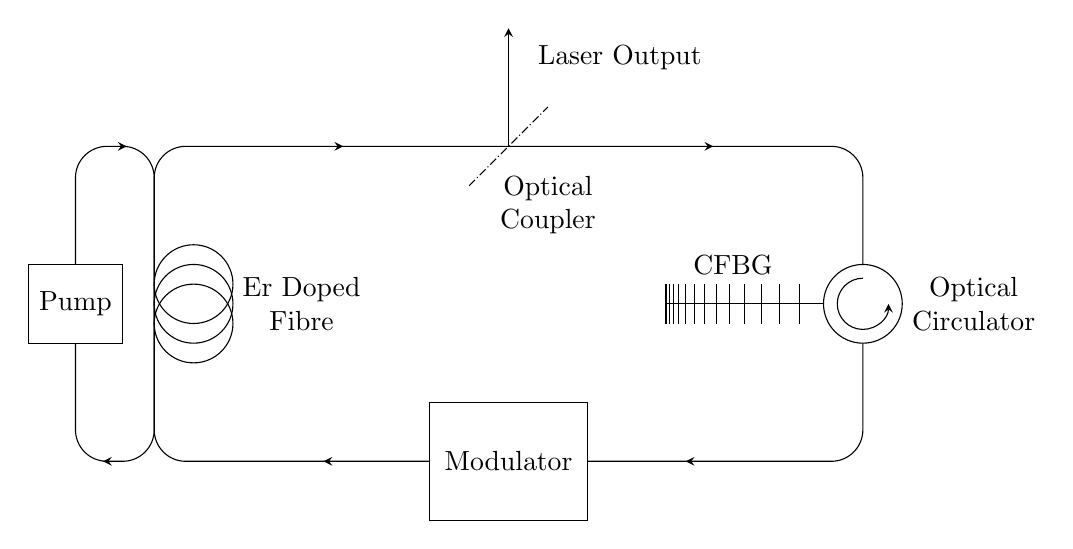
\begin{tikzpicture}
% Two laser loops
\draw [rounded corners=4mm] (0,0) rectangle ++(9,4);
\draw [rounded corners=4mm] (0,0) rectangle ++(-1,4);

% Gain
\draw (0.5,2.25) circle (0.5cm);
\draw (0.5,2) circle (0.5cm) node [anchor=west,xshift=0.5cm,align=center] {Er Doped \\ Fibre};
\draw (0.5,1.75) circle (0.5cm);

% Modulator and pump
\filldraw[fill=white, draw=black] (3.5,-0.75) rectangle ++(2,1.5) node [midway] {Modulator};
\filldraw[fill=white, draw=black] (-1.6,1.5) rectangle ++(1.2,1) node [midway] {Pump};

% Coupler and output
\draw[-stealth] (4.5,4) -- (4.5,5.5) node [pos=0.75,anchor=west,xshift=0.25cm] {Laser Output};
\draw[densely dashdotted] (4,3.5) -- (5,4.5) node [pos=1,anchor=north,yshift=-0.75cm,align=center] {Optical \\ Coupler};

% Circulator
\filldraw[fill=white, draw=black] (9,2) circle (0.5cm) node [anchor=west,xshift=0.5cm,align=center] {Optical \\ Circulator};
\draw[->,>=stealth] (9,2.325) arc (90:360:0.325cm);

% Grating
\draw (8.5,2) -- (6.5,2) node [pos=0.5,anchor=south,yshift=0.25cm,xshift=-0.15cm] {CFBG};
\foreach \i in {0,...,13}
  \draw (6.5 + \i*\i/100,1.75) -- (6.5 + \i*\i/100,2.25);

% Arrows
\draw[-stealth] (2.16,0) -- (2.15,0);
\draw[-stealth] (2.39,4) -- (2.4,4);
\draw[-stealth] (6.76,0) -- (6.75,0);
\draw[-stealth] (7.09,4) -- (7.1,4);
\draw[-stealth] (-0.649,0) -- (-0.65,0);
\draw[-stealth] (-0.351,4) -- (-0.35,4);H
\end{tikzpicture}
	\caption{Typical cavity of a fibre ring laser~\cite{burgoyne2014, chung2017, lapre2019, shao2019}. The pump laser travels clockwise around the left-hand loop (red arrows) energizing the Er-doped fibre. The main laser travels clockwise around the right-hand loop (blue arrows) passing through each component, with most of the pulse exiting the cavity through the optical coupler.}
	\label{fig:cavity}
\end{figure}

The canonical equation in nonlinear optics is the nonlinear Schr\"odinger equation (NLSE),
\begin{align}
	\pdiff{A}{z} &= - i \frac{\beta_2}{2}\pdiff[2]{A}{T} + i \gamma |A|^2 A.
	\label{eq:smallnlse}
\end{align}
Here, $A = A(T, z)$ is the complex pulse envelope, $T$ is co-moving time, $z$ is the propagation coordinate, and $\beta_2$ and $\gamma$ are the group velocity dispersion and Kerr nonlinearity, respectively. Typically, \eqref{eq:smallnlse} is generalized to incorporate terms more specific to laser physics. A gain term and loss term are added (and sometimes higher order dispersion), to give the generalized nonlinear Schr\"odinger equation (GNLSE)~\cite{agrawal2013, bohun2015, finot2008, peng2018, shtyrina2017, yarutkina2013},
	\begin{align}
	\pdiff{A}{z} &= - i \frac{\beta_2}{2}\pdiff[2]{A}{T} + i \gamma |A|^2 A + \frac{1}{2}g(A) A - \alpha A,
	\label{eq:nlse}
\end{align}
where $g(A)$ is an amplifying term due to the gain fibre, and $\alpha$ is the loss due to scattering and absorption.

The GNLSE, \eqref{eq:nlse}, has many applications in nonlinear optics and fibre optic communications, however, it is regularly generalized further to include a modulation term in the context of lasers. The resulting equation is referred to as the master equation of mode-locking (see \cite{haus1975, haus1984, haus2000, tamura1996, usechak2005}), or sometimes the Ginzburg--Landau equation. Due to the nonlinear term in \eqref{eq:nlse} and the often non-trivial form of $g(A)$, as well as the possible addition of a modulation term, no analytic solution is known. See Haus~\cite{haus2000} for a comprehensive description and history of the theory of mode-locked lasers. The GNLSE well represents the dynamics in, say, a single optical fibre, it is not entirely representative of the underlying physics within a laser cavity. It is assumed in \eqref{eq:nlse} that each process affects the pulse continuously within the cavity. Therefore, the GNLSE, and its derivatives, can be thought of as an `average' model for lasers---this assumption breaks down if the pulse undergoes large changes during one round trip. Often, this is the case due to the specialized, discrete components.

In this paper, we will build an iterative map model for the evolution of a laser pulse as it travels though the cavity. In Section~\ref{sec:model}, we will briefly review previous iterative mathematical models, then, we will derive our own iterative map model from \eqref{eq:nlse}. We will then non-dimensionalize the model and introduce four dimensionless parameters that govern the dynamics of the system. We will then examine the results of our model in Section~\ref{sec:results}---first solving the model analytically, by assuming the absence of the nonlinearity, then numerically solving the full nonlinear model. We will identify a sharp boundary in the parameter space separating the region of stability, and the region where modulation instability degrades the pulse. Finally, the concluding thoughts and possible ideas for future work are given in Section~\ref{sec:conclusion}.

\section{Iterative Map Model}
\label{sec:model}
To resolve some of the issues with an `average' model, it is common to use separate GNLSEs for each component and region in the laser, iteratively passing the pulse from one PDE to the next \cite{lapre2019, meng2020, oktem2010, woodward2018}. This method allows us to better encapsulate specific dynamics introduced by each component. The main drawback of this method is its extreme computational expense, since a nonlinear PDE must be numerically solved for every component and each of the hundreds of round trips in a given simulation. We can alleviate this computational expense by noticing that each effect is localized to its corresponding component in the cavity: essentially all of the dispersion happens within the CFBG~\cite{agrawal2002}, the pulse is only amplified within the Er-doped fibre, \emph{et cetera}. Therefore, we can drastically simplify each of the GNLSEs into a form we can solve analytically. We get the benefit of the fine-grain simulation over an `average' model, allowing us to reflect the specific geometry of the cavity, without much additional computational cost.

Iterative map methods have been around since 1955 when Cutler~\cite{cutler1955} analyzed a microwave regenerative pulse generator. Siegman and Kuizenga~\cite{kuizenga1970a, kuizenga1970b, kuizenga1970, siegman1969} adapted Cutler's method for both AM and FM mode-locked lasers in 1969, and Martinez \emph{et al.}~\cite{martinez1984, martinez1985} incorporated the nonlinearity while modelling passively mode-locked lasers. This method was used for dispersion-tuned actively mode-locked lasers recently by Burgoyne \emph{et al.}~\cite{burgoyne2014}. Each of these models used a prescribed transfer function to describe the effect each component has on the pulse. While the transfer functions are chosen suitably to have the effect observed in the laboratory, they are phenomenologically chosen, and not necessarily obtained from the underlying physics. Furthermore, these methods have not included the effect of every component, lacking the imperative interplay of dispersion, modulation, and nonlinearity---disallowing their models to exhibit modulation instability.

We continue by deriving our own iterative map model by solving a reduced GNLSE for each component---except modulation, which we consider to be applied externally by an electro-optic modulator. Within the gain fibre, we assume all other effects are negligible, allowing us to simplify \eqref{eq:nlse} to
\begin{align}
	\pdiff{A}{z} &= \frac{1}{2}g(A)A.
	\label{eq:gainexample}
\end{align}
To proceed, we assume the gain has the form
\begin{align}
	g(A) &= \frac{g_0}{1 + E / \Es},& E &= \int_{-\infty}^\infty |A|^2 \, \df T,
	\label{eq:energy}
\end{align}
where $g_0$ is a small signal gain, $E$ is the energy of the pulse, and $\Es$ is the energy at which the gain begins to saturate~\cite{haus1984, shtyrina2017, silfvast2004}, which depends on the power of the pump laser. Thus, \eqref{eq:gainexample} becomes
\begin{align}
	\pdiff{A}{z} &= \frac{g_0 A}{2 \left( 1 + E / \Es \right)}.
\end{align}
By assuming the energy entering the gain fibre is $E_g$ and the energy after travelling through the gain fibre of length $L_g$ is $E_{\text{out}}$, we find the energy after amplification is
\begin{align}
	\label{eq:engain}
	E_{\text{out}} &= \Es W \left( \frac{E_g}{\Es} \exp( E_g / \Es ) \exp( g_0 L_g ) \right),
\end{align}
where $W$ is the Lambert $W$ function. Rewriting \eqref{eq:engain} in terms of the pulse gives
\begin{align}
	G(A) &= \left( \frac{\Es}{E_g} W \left( \frac{E_g}{\Es} \exp( E_g / \Es ) \exp( g_0 L_g ) \right) \right)^{1/2} A
	\label{eq:gainform}
\end{align}
for the amplification of the pulse within the Er-doped fibre.

Repeating this same procedure for the loss, dispersion, and nonlinearity yields
\begin{align}
	L(A) &= (1 - R) \exp( - \alpha L_T )A, \\
	D(A) &= \FTi{\exp( i \omega^2 L_D\beta_2/2 ) \FT{A}}, \\
	F(A) &= A \exp( i \gamma |A|^2 L_f ),
\end{align}
where $R$ is the reflectivity of the optical coupler (depending on the layout of the laser cavity the loss may instead take the form $L(A) = R \exp( - \alpha L_T )A$), $L_T$ is the total length of the laser circuit, $L_D$ is the length of the dispersive medium, $L_f$ is the length of fibre between the amplifier and the optical coupler, and $\mathcal{F}$ denotes the Fourier transform. Finally, we consider the modulation. Here, we assume the pulse is modulated by an electro-optic modulator. This gives the freedom of choosing the profile of the modulation how ever the operator sees fit. For simplicity the representation is taken as the Gaussian
\begin{align}
	M(A) &= \exp( -T^2 / 2 T_M^2 ) A,
	\label{eq:modform}
\end{align}
where $T_M$ is the characteristic width of the modulation. This assumption is not particularly restrictive. Calcaterra and Boldt~\cite{calcaterra2008a} have shown that a sum of Gaussian functions can approximate any square integrable function. Therefore, our solution extends to any continuous, bounded modulation function. Additionally, it is common to use a saturable absorber in place of a modulator. In this case, \eqref{eq:modform} can freely be replaced by~\cite{lapre2019, meng2020, oktem2010, woodward2018}
\begin{align}
	S(A) &= 1 - \frac{q_0}{1 + |A|^2 / P_\text{sat}},
\end{align}
where $q_0$ is the modulation depth, $|A|^2$ is the instantaneous power of the pulse, and $P_\text{sat}$ is the saturation power.

\subsection{Non-Dimensionalization}
Non-dimensionalization is a technique used in mathematical modelling to better understand the relative importance of different processes within a system. In essence, we scale all variables by typical values of the system based on the geometry and boundary conditions (see, for example,~\cite{howison2005}). Doing so `factors' the dimensional units out of the problem, leaving only dimensionless equations with dimensionless parameters. The magnitude of the dimensionless parameters characterizes the dominant dynamics of the system---much like how fluid flow can be described with only the Reynolds number. The structure of each process in the laser can be better understood by re-scaling the time, energy, and amplitude by the convenient scalings:
\begin{align}
	T &= T_M \widetilde{T},& E &= \Es \widetilde{E},& A &= \left( \frac{\Es}{T_M} \right)^{1/2} \widetilde{A}.
\end{align}

Returning to the process maps \eqref{eq:gainform}--\eqref{eq:modform}, we find the non-dimensional mappings to be (after dropping the tildes)
\begin{align}
	G(A) &= \left(E_g^{-1} W \left( a E_g \textrm{e}^{E_g}\right) \right)^{1/2} A, & F(A) &= A \exp( i b |A|^2), \nonumber \\
	D(A) &= \FTi{\exp( i s^2 \omega^2 ) \FT{A}}, & L(A) &= h A, \label{eq:effects} \\
	M(A) &= \exp( -T^2 / 2 ) A, \nonumber
\end{align}
with the four dimensionless parameters,
\begin{equation}
	\begin{aligned}
		a &= \exp( g_0 L_g ) \sim 8 \times 10^3, & 
		h &= (1 - R) \exp( - \alpha L_T) \sim 0.04, \\
		b &= \gamma L_f \frac{\Es}{T_M} \sim 1, & s &= \left( \frac{\beta_2 L_D}{2 T_M^2} \right)^{1/2} \sim 0.2,
		\label{eq:ndparam}
	\end{aligned}
\end{equation}
as defined by the values in Table~\ref{tab:values}. Here, $a$ is a measure of the strength of the gain fibre, $h$ is the loss due to absorption and the optical coupler, $b$ is the ratio of the frequency shift due to the Kerr nonlinearity to the width of the pulse, and $s$ is the ratio of the effectiveness of the CFBG to the width of the pulse. Furthermore, notice that in this non-dimensional form, the modulation has no associated parameter, and each of the other processes in \eqref{eq:ndparam} have their own independent, non-dimensional parameter.

% Table of parameter values
\begin{table*}[tbp]
	\centering
	\caption{Range of parameter values (taken from~\cite{agrawal2013, burgoyne2014, burgoyneemail, tamura1996, usechak2005}).}
 	\label{tab:values}
 	\begin{tabular}{clll}
		\hline\noalign{\smallskip}
		Symbol & Parameter & Value & Units \\
		\hline\noalign{\smallskip}
		$T_M$ & Characteristic modulation time & $15$--$150$ & ps \\
		$\beta_2^g L_D$ & Dispersion provided by CFBG & $10$--$2000$ & ps$^2$ \\
		$\gamma$ & Kerr nonlinearity coefficient & $0.001$--$0.01$ & W$^{-1}$ m$^{-1}$ \\
		$L_f$ & Length of fibre between gain and optical coupler & $0.15$--$1$ & m \\
		$L_g$ & Length of the Er-doped gain fibre & $2$--$3$ & m \\
		$\alpha$ & Loss of fibre due to scattering and absorption & $10^{-4}$--$0.3$ & m$^{-1}$ \\
		$R$ & Reflectivity of optical coupler & $0.1$--$0.9$ & -- \\
		$\Es$ & Saturation energy of Er-doped gain fibre & $10^3$--$10^4$ & pJ \\
		$\beta_2^f$ & Second order fibre dispersion & $-50$--$50$ & ps$^2$/km \\
		$g_0$ & Small signal gain &  $1$--$10$ & m$^{-1}$ \\
		$L_T$ & Total length of fibre in the cavity & $10$--$100$ & m \\
		\noalign{\smallskip}\hline
	\end{tabular}
\end{table*}

\subsection{Combining the Effects}
\label{sec:effects}

\begin{figure}[tbp]
	\centering
	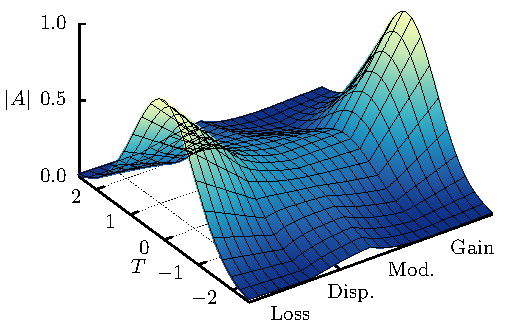
\includegraphics{Figures/Evo}
	\caption{Evolution of the envelope during one round trip of the cavity at equilibrium. The pulse decays due to the optical coupler, disperses due to the CFBG, is modulated by the modulator, and finally, is amplified by the gain fibre (the envelope is unaltered by the nonlinearity). Note, the $z$ axis is not to scale.}
	\label{fig:cavityevo}
\end{figure}

Now that we have the algebraic effect of each section of the cavity, we are ready to take the composition of the maps to give the effect of one round trip of the cavity. Unlike the models models described in the beginning of this section, the permutation of our components is important as the maps \eqref{eq:effects} do not commute with each other. Furthermore, the order of the components will be dictated by the geometry of a particular laser, however, we the laser is constructed as in Fig.~\ref{fig:cavity},  with the following justifications. The effect of the nonlinearity will me maximized after the pulse passes through the gain fibre---this is the region where the pulse is most energetic. Thus, we take the nonlinearity component to follow the gain. Similarly, we would want the loss component to directly follow the nonlinearity in an attempt to minimize the effect the nonlinearity has on the pulse. This leaves the dispersion and modulation components. For now, let us assume the CFBG precedes the modulator. Finally, we assume the loss component is our reference point since this corresponds to the optical coupler, and thus, the point in the cavity we are able to take our measurements. More precisely, let
\begin{align}
	\mathcal{L}(A) = F(G(M(D(L(A)))))
	\label{eq:order}
\end{align}
denote one complete round trip of the cavity. Since a ring laser is cyclic in nature, we use the result of one round trip as the input pulse for the next round trip---restarting the process. We continually repeat this procedure until the envelope and chirp of the pulse reaches equilibrium, or the pulse degrades due to modulation instability. Note that we are uninterested in the phase change as it is not modified by the maps in a meaningful way, and due to the nature of experimental measurements. An example of the evolution of the envelope during one round trip of the laser cavity can be found in Fig.~\ref{fig:cavityevo}.

\section{Results}
\label{sec:results}
We split the results into two subsections. In the following subsection we investigate the low nonlinearity limit, and in Section~\ref{sec:results}\ref{sec:nlresults} we look at the full nonlinear model.

\subsection{Linear Solution}
By neglecting the effect of the nonlinearity, that is, $b = 0$, a solution can be found analytically. We proceed by assuming a fixed point will take the form of a linearly chirped Gaussian. There are a few reasons for this; the solution to the models presented in~\cite{cutler1955, siegman1969, kuizenga1970a, martinez1984, martinez1985} were Gaussian, the equilibrium shape will be highly correlated to the modulation function, and since a Gaussian is a fixed point of the Fourier transform. Furthermore, this form is chosen because it resembles the envelope and linear chirp expected from the literature~\cite{burgoyne2014, haus1975, haus1996, haus2000, usechak2005}.

\begin{figure}[tbp]
	\centering
	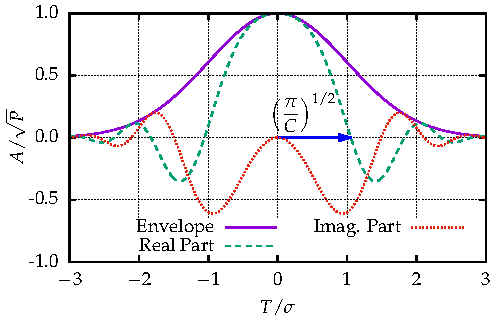
\includegraphics{Figures/Sample_Gauss}
	\caption{Linearly chirped Gaussian pulse, \eqref{eq:A0}.}
	\label{fig:samplegauss}
\end{figure}

\begin{figure*}[tbp]
	\centering
	\begin{subfigure}{\columnwidth}
		\centering
		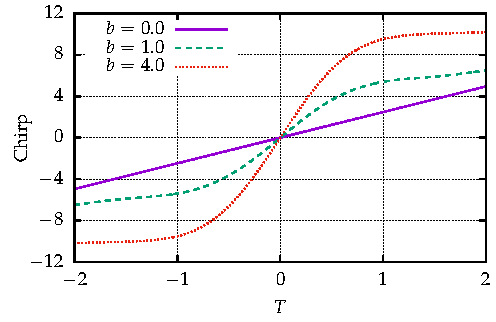
\includegraphics{Figures/Chirp}
		\caption{Chirp.}
		\label{fig:chirp}
	\end{subfigure} %
	\begin{subfigure}{\columnwidth}
		\centering
		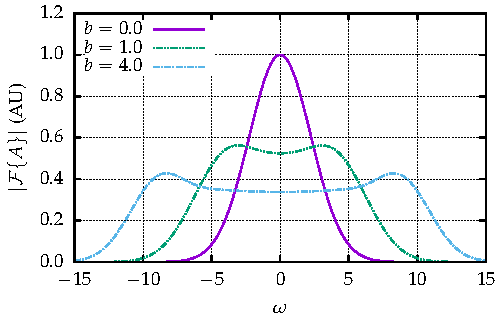
\includegraphics{Figures/FT}
		\caption{Fourier transform.}
		\label{fig:ft}
	\end{subfigure}
	\caption{Chirp and Fourier transform at equilibrium (500 round trips) initiated by \eqref{eq:nlA0} for two values of $b$, the nonlinearity parameter ($a = 8 \times 10^3$, $h = 0.04$, $s = 0.2$, and $E_0 = 0.1$).}
	\label{fig:chirpft}
\end{figure*}

Consider the pulse
\begin{align}
	A = \sqrt{P} \exp \left( -(1 + iC) \frac{T^2}{2 \sigma^2} \right) \textrm{e}^{i \phi_0},
	\label{eq:A0}
\end{align}
where $P$ is the peak power, $C$ is the chirp, $\sigma^2$ is the variance, and $\phi_0$ is the phase (Fig.~\ref{fig:samplegauss}). By computing $\mathcal{L}(A)$ using \eqref{eq:order}, and equating to $A \textrm{e}^{i \phi}$, we obtain the conditions
\begin{align}
	\frac{\sigma^4}{1 - \sigma^2} &= (\sigma^2 + 2 C s^2)^2 + 4 s^4, \label{eq:sigrelation} \\
	\frac{C}{1 - \sigma^2} &= C + 2 \frac{s^2}{\sigma^2} (1 + C^2), \label{eq:chirprelation} \\
	1 &= \frac{W(a E_g \textrm{e}^{E_g})}{E_g} h^2 (1 - \sigma^2)^{1/2} \label{eq:energyrelation}
\end{align}
for \eqref{eq:A0} to be in equilibrium. Manipulating \eqref{eq:sigrelation} and \eqref{eq:chirprelation} we are able to eliminate the chirp, and find an expression in terms of $\sigma$ only, that is,
\begin{align}
	\sigma^8 + 4 s^4 \sigma^6 - 20 s^4 \sigma^4 + 32 s^4 \sigma^2 - 16 s^4 = 0. \label{eq:var}
\end{align}
As \eqref{eq:var} is a quartic in $\sigma^2$, it has an analytic solution, namely,
\begin{equation}
	\begin{split}
		\sigma^2 = \sqrt{2} s \left( s^6 + 3s^2 + \sqrt{4 + s^4} \left( 1 + s^4 \right) \right)^{1/2} & \\
		- s^4 - s^2 & \sqrt{4 + s^4}.
		\label{eq:equilvar}
	\end{split}
\end{equation}
Additionally, we find the chirp to be
\begin{align}
	C = \frac{\sigma^4 - \left( \sigma^8 - 16 s^4 \left( 1 - \sigma^2 \right)^2 \right)^{1/2}}{4 s^2 \left( 1 - \sigma^2 \right)},
	\label{eq:chirp}
\end{align}
in terms of $s$ and $\sigma^2$. Moreover, we can obtain the energy of the pulse entering the gain fibre, $E_g$, from \eqref{eq:energyrelation}, and thus, the equilibrium energy at the optical coupler. Doing so gives
\begin{align}
	E &= \frac{\log \left( a h^2 \left( 1 - \sigma^2 \right)^{1/2} \right)}{1 - h^2 \left( 1 - \sigma^2 \right)^{1/2}}.
	\label{eq:analenergy}
\end{align}
By equating the energy of the pulse in \eqref{eq:A0} and \eqref{eq:analenergy}, the peak power is found to be
\begin{align}
	P &= \frac{\log \left( a h^2 \left( 1 - \sigma^2 \right)^{1/2} \right)}{\sqrt{\pi} \sigma \left( 1 - h^2 \left( 1 - \sigma^2 \right)^{1/2} \right)}.
	\label{eq:analpower}
\end{align}

The nature of \eqref{eq:var}--\eqref{eq:analpower} makes it difficult to work with. However, by asymptotically expanding \eqref{eq:var}--\eqref{eq:analpower} in terms of the dispersion parameter, $s$, we find the simpler relations
\begin{align}
	\sigma^2 &\sim 2s(1 - s) + \bigO{s^3}, \\
	C &\sim 1 - s + \frac{1}{2}s^2 + \bigO{s^3}, \\
	E &\sim \frac{\log (a h^2)}{1 - h^2} - \frac{1}{1 - h^2} \left( 1 + \frac{h^2 \log(a h^2)}{1 - h^2}  \right) s + \bigO{s^2}, \label{eq:maxenergy} \\
	P &\sim \frac{\log(ah^2)}{\sqrt{2 \pi}(1 - h^2)} s^{-1/2} + \bigO{s^{1/2}},
\end{align}
in the case $s \rightarrow 0$. And,
\begin{align}
	\sigma^2 &\sim 1 - \frac{1}{4}s^{-4} + \frac{3}{8}s^{-8} + \bigO{s^{-12}}, \label{eq:siginfty}\\
	C &\sim \frac{1}{2}s^{-2} - \frac{3}{8}s^{-6} + \bigO{s^{-10}},
\end{align}
in the case $s \rightarrow \infty$. We have no asymptotic expansion of the energy or peak power as $s \rightarrow \infty$ since in this limit the gain is unable to balance the energy lost due to modulation, as indicated by the logarithm in \eqref{eq:analenergy}. Expanding the condition $a h^2 (1 - \sigma^2)^{1/2} > 1$, from \eqref{eq:analenergy}, using \eqref{eq:siginfty} (for a first-order approximation), we find 
\begin{align}
	s^* = \left( \frac{a h^2}{2} \right)^{1/2}
\end{align}
is the maximum value of $s$ to facilitate a sustainable pulse.

Our linearized model indeed exhibits a solution of the same form as previous linear models. However, by including the effects of the nonlinearity we uncover the rich interplay between dispersion, modulation, and nonlinearity.

\subsection{Nonlinear Solution and Instability}
\label{sec:nlresults}
In this iterative map model---as well as within the laboratory---we must specify the input pulse. One of the most common forms is a hyperbolic secant~\cite{coen1997, finot2008, rothenberg1989b, tomlinson1984}, which we assume has the exact form
\begin{align}
	A_0 = \Gamma \sech \left( 2 T \right) \textrm{e}^{i \pi / 4},
	\label{eq:nlA0}
\end{align}
where $\Gamma$ is a normalizing factor chosen so the pulse has the initial energy $E_0$, which we take as $E_0 = 0.1$, unless specified otherwise. Using \eqref{eq:nlA0} as a seed, we simulate the pulse as it travels around the cavity using $2^{18}$ points, and a time span of 16.

In Fig.~\ref{fig:chirpft} we show the chirp and Fourier transform of the pulse \eqref{eq:nlA0} once it has reached equilibrium for the nominal parameter values given in \eqref{eq:ndparam}, and an additional $b$ value. In this nonlinear case, we find that the equilibrium pulse is no longer Gaussian---as evidenced by the Fourier transforms. Notice that compared to the linear case, higher frequency modes are introduced due to the nonlinearity, giving a bi-modal appearance. Moreover, we find the pulse is linearly chirped near the peak, but, in the tails, $|T| > 1$, the chirp begins to saturate---consistent with the experimental results~\cite{chen2008, rothenberg1989b, tomlinson1985}. As the nonlinearity parameter, $b$, is increased, the chirp increases more sharply across the pulse, and saturates at a larger value. Also, the two lobes in the Fourier transform become more pronounced and further apart, and the pulse becomes more rectangular. However, after a critical point, SPM plays a more substantial role, leading to modulation instability. This phenomenon is highlighted in Fig.~\ref{fig:breakevo}. By increasing the nonlinearity, and decreasing the dispersion we find the pulse begins to `breathe'. During the first two dozen round trips of the cavity, the SPM compounds and becomes too parasitic to the pulse. This in turn induces modulation instability, and degrades the pulse, until the pulse is no longer stable or sustainable. On the other hand, having a more moderate value of $b$, the pulse is able to equilibrate even with a less favourable, random, initial pulse (Fig.~\ref{fig:convevo}), as in~\cite{meng2020}. The pulse is able to shed the initial left lobe ($T = -1 / 2$) because of dispersion and modulation, and a central lobe ($T = 0$) is formed and is able to grow due to the gain medium. This then allows the pulse to come to equilibrium very quickly. Furthermore, since the intensity of the initial pulse is relatively small, the effect of SPM is negligible during the first few round trips which allows the laser to select preferable modes. The preferable modes then get amplified which stabilizes the pulse. From this, it is clear the initial shape of the pulse is much less important than the initial energy of the pulse, $E_0$, or the strength of the nonlinearity, $b$.

\begin{figure}[tbp]
	\centering
	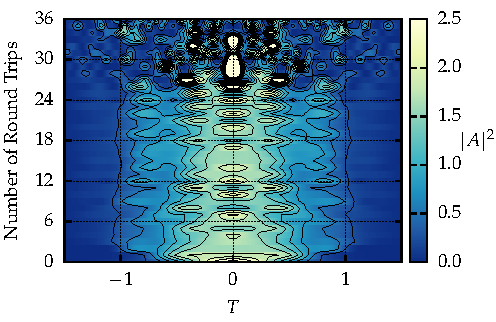
\includegraphics{Figures/Break}
	\caption{Example of a pulse destabilizing from the initial pulse \eqref{eq:nlA0} ($a = 8 \times 10^3$, $h = 0.04$, $b = 1.6$, $s = 0.1$, and $E_0 = 0.1$).}
	\label{fig:breakevo}
\end{figure}

\begin{figure}[tbp]
	\centering
	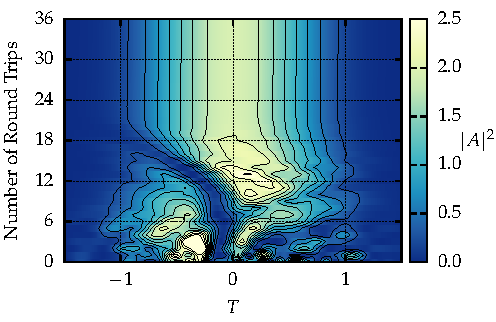
\includegraphics{Figures/Conv}
	\caption{Example of a pulse coming to equilibrium from noise ($a = 8 \times 10^3$, $h = 0.04$, $b = 1.0$, $s = 0.1$, and $E_0 = 0.1$).}
	\label{fig:convevo}
\end{figure}

We now turn our attention to a more quantitative analysis, and characterize the stability of a laser by exploring the parameter space. We focus on the $s$--$b$ plane in particular since $a$ and $h$ effect only the amplitude of the pulse, whereas the interplay of dispersion and nonlinearity give rise to the instabilities. Additionally, as mentioned, a conservative initial energy will effect the dynamics much less than a more intense pulse since the nonlinearity will be negligible while coming to equilibrium. To identify the stability of a pulse we examine the relative change in the pulse's envelope between consecutive round trips of the cavity. We compute this error by
\begin{align}
	\Delta = \frac{\| |\mathcal{L}^n(A_0)| - |\mathcal{L}^{n-1}(A_0)| \|_2}{\| \mathcal{L}^{n-1}(A_0) \|_2},
	\label{eq:error}
\end{align}
where
\begin{align}
	\| f \|_2^2 \coloneqq \int_{-\infty}^\infty |f|^2 \, \df T,
\end{align}
and $n$ is chosen to be sufficiently large to guarantee the pulse reaches equilibrium or degrades due to modulation instability---we use $n = 500$ in our experiments. We take the modulus of the pulse since we are only interested in the evolution of the envelope because of the methods used experimentally. We plot the error in Fig.~\ref{fig:error}. It is clear the parameter space is split into two distinct regions, divided by an incredibly sharp and complex boundary. In the upper-left region the error is $\bigO{1}$; here, the nonlinearity is too strong, and the SPM induces modulation instability. In the lower-right region we find the opposite behaviour---the pulse reaches an equilibrium state and is stable. The increase in dispersion, coupled with modulation, allows the laser to balance the nonlinear effects. The error in this region is on the order of machine precision, or slightly higher due to the discretization.

\begin{figure}[tbp]
	\centering
	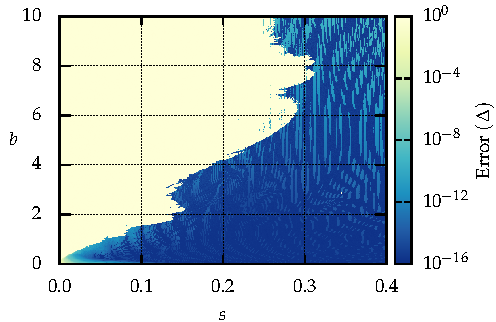
\includegraphics{Figures/ParamSpaceErr}
	\caption{Relative error of a pulse's envelope between round trips 499 and 500 ($a = 8 \times 10^3$, $h = 0.04$, and $E_0 = 0.1$).}
	\label{fig:error}
\end{figure}

Also of interest is the energy of the pulse at equilibrium, which we compute numerically by \eqref{eq:energy}. Recall from \eqref{eq:order}, this energy is immediately before passing through the optical coupler, and so the energy of each pulse emitted by the laser is $(1 - h^2) E$, and $h^2 E$ remains in the cavity. We plot the energy in the $s$--$b$ plane in Fig.~\ref{fig:energy}. Unsurprisingly, we find the same sharp boundary as we saw in Fig.~\ref{fig:error}. In the unstable region (upper-left) the energy is relatively small. Since the pulse is not sustainable in this region it is not able to foster prominent modes, thus, the intensity is low across the entire pulse. In the stable region (lower-right) we find that the energy smoothly decays as both $b$ and $s$ increase, with the contours being hyperbolic-esque. As $s$ increases, more energy is lost due to modulation since the tails of the pulse become larger. Similarly, as $b$ increases, high frequencies generated by SPM are reduced by our choice of modulation function. From this, we find that a more energetic laser requires weaker dispersion, however, the nonlinearity must be correspondingly low, otherwise modulation instability will destroy the pulse. Moreover, the maximum energy, which occurs in the limit that both $s$ and $b$ go to zero, is slightly larger than 2.5. With our choice of parameters, \eqref{eq:maxenergy} predicts an energy of 2.55 at the origin, inline with Fig.~\ref{fig:energy}.

\begin{figure}[tbp]
	\centering
	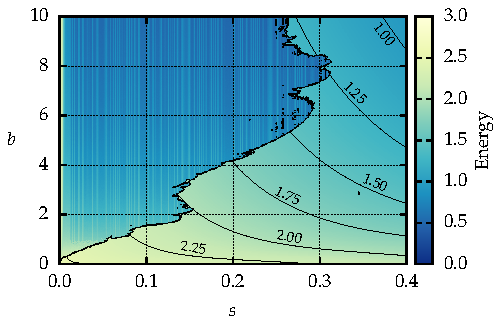
\includegraphics{Figures/ParamSpaceEnergy}
	\caption{Energy of the pulse after 500 round trips ($a = 8 \times 10^3$, $h = 0.04$, and $E_0 = 0.1$).}
	\label{fig:energy}
\end{figure}

Finally, we briefly investigate the effect the order of the components has on the dynamics. In Section~\ref{sec:model}\ref{sec:effects} we justified the order of the gain, nonlinearity, and loss, but, just assumed dispersion preceded modulation. Here, we consider the effect of swapping the dispersion and modulation components. The energy landscape (Fig.~\ref{fig:energyswitch}) is as we would expect. In the previous case of having modulation following dispersion, more energy is removed from the pulse tails. Whereas, having modulation first, more of this energy remains in the cavity. This has the effect of making the laser more powerful than in the previous case, which in turn increases the size of the unstable region. Comparing with Fig.~\ref{fig:energy}, the unstable upper-left region spreads farther rightward, and the energy is larger in the stable region---especially farther away from the origin. Lastly, once again, the energy at the origin is somewhat larger than 2.5, as predicted by \eqref{eq:maxenergy}.

\begin{figure}[tbp]
	\centering
	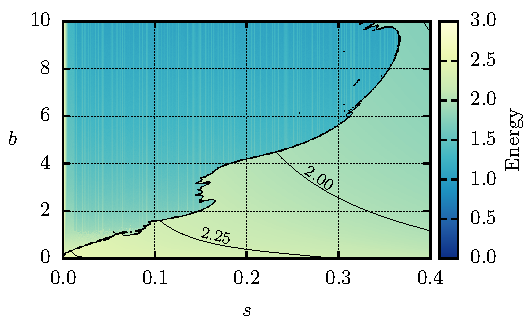
\includegraphics{Figures/ParamSpaceEnergySwitch}
	\caption{Energy of the pulse after 500 round trips with dispersion and modulation swapped ($a = 8 \times 10^3$, $h = 0.04$, and $E_0 = 0.1$).}
	\label{fig:energyswitch}
\end{figure}

\section{Conclusion}
\label{sec:conclusion}
Expanding upon the ideas originally proposed by Cutler~\cite{cutler1955}, and Kuizenga and Siegman~\cite{kuizenga1970, kuizenga1970a, siegman1969}, we developed a nonlinear iterative map model for tuneable ring lasers. We recovered linearly chirped Gaussian solutions in the case of a Gaussian modulation function when omitting the nonlinearity. Moreover, the solution of the linear model can easily be extended to any modulation function using results of~\cite{calcaterra2008a}. In contrast, with the inclusion of the nonlinearity we were able to recover wave breaking and modulation instability, and found a sharp boundary of stability. This phenomenon has been demonstrated in a laboratory setting~\cite{agrawal2013, anderson1992, finot2008, rothenberg1989b, tomlinson1985}, but, has proven difficult to predict with simple mathematical models~\cite{meng2020}. We've shown that a simple iterative map model is able to reproduce complicated instabilities arising naturally from the interplay between dispersion, modulation, and nonlinear effects. Our model can easily be adapted to specific laser geometries, and to more complicated models of the components. For example, incorporating a frequency dependence in the gain function, or using a saturable absorber instead of a Gaussian modulator.

It is of interest to analyze the nonlinear model analytically using an asymptotic expansion for small values of the nonlinearity parameter, $b$. Doing so would provide insight to how the nonlinearity impacts the linearized solution to better understand the manifestation of wave breaking and modulation instability. Furthermore, a more detailed analysis of crossing the sharp boundary between stability and instability may provide valuable insight for mechanisms that trigger the instability.

\section*{Acknowledgement.}

Portions of this work were presented at The V AMMCS International Conference in 2019, ``A new method of modelling tuneable lasers with functional composition'' \cite{metherallammcs}. BM acknowledges the support provided by the EPSRC Centre for Doctoral Training in Industrially Focused Mathematical Modelling (EP/L015803/1).

%The authors would like to thank O. Aytür for critical reading of the manuscript

\section*{Disclosures.}
The authors declare no conflicts of interest.

\bibliography{Ref}

\end{document}
